%%%%%%%%%%%%%%%%%%%%%%%%%%%%%%%%%%%%%%%%%%%%%%%%%%%%%%%%%%%%%%%%%%%%%
% LaTeX Template: Project Titlepage Modified (v 0.1) by rcx
%
% Original Source: http://www.howtotex.com
% Date: February 2014
% 
% This is a title page template which be used for articles & reports.
% 
% This is the modified version of the original Latex template from
% aforementioned website.
% 
%%%%%%%%%%%%%%%%%%%%%%%%%%%%%%%%%%%%%%%%%%%%%%%%%%%%%%%%%%%%%%%%%%%%%%

\documentclass[12pt]{article}
\usepackage[a4paper]{geometry}
\usepackage[myheadings]{fullpage}
\usepackage{fancyhdr}
\usepackage{lastpage}
\usepackage{graphicx, wrapfig, subcaption, setspace, booktabs}
\usepackage[utf8]{inputenc}
\usepackage[T1]{fontenc}
\usepackage[font=small, labelfont=bf]{caption}
\usepackage{fourier}
\usepackage[protrusion=true, expansion=true]{microtype}
\usepackage[french]{babel}
\usepackage{caption}
\usepackage{sectsty}
\usepackage{url, lipsum}
\usepackage{amsmath}



\usepackage{tikz}
\usepackage[most]{tcolorbox}
\usepackage[pstricks]{bclogo}
\usepackage{pst-blur}




\newcommand{\HRule}[1]{\rule{\linewidth}{#1}}
\onehalfspacing
\setcounter{tocdepth}{5}
\setcounter{secnumdepth}{5}

%-------------------------------------------------------------------------------
% HEADER & FOOTER
%-------------------------------------------------------------------------------
\pagestyle{fancy}
\fancyhf{}
\setlength\headheight{15pt}
\fancyhead[L]{BTS CPRP 1}
\fancyhead[R]{Lycée Le Corbusier}
\fancyfoot[R]{Page \thepage\ sur \pageref{LastPage}}
\fancyfoot[L]{TP - Industrialisation}
%-------------------------------------------------------------------------------
% TITLE PAGE
%-------------------------------------------------------------------------------
 
 

%%%%POUR FAIRE DES EXERCICES INDÉPENDAMMENT DES SECTIONS%%%%
%%%%%%%%%%%%%%%%%%%%%%%%%%%%%%%%%%%%%%%%%%%%%%%%%%%%%%%%%%%%%%%%%%%
\newcounter{exo}
\newenvironment{exo}{\stepcounter{exo}\vspace{0.5cm}{\bfseries Question \theexo\ :}}{\par\vspace{0.5cm}}
%%%%%%%%%%%%%%%%%%%%%%%%%%%%%%%%%%%%%%%%%%%%%%%%%%%%%%%%%%%%%%%%%%%%




\begin{document}
 
\title{ 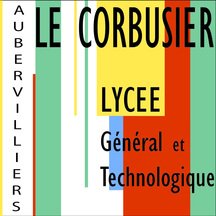
\includegraphics[width=0.18\linewidth]{corbu.jpg} \hspace{2cm} \normalsize \textsc{TP Industrialisation noté \hspace{2cm} 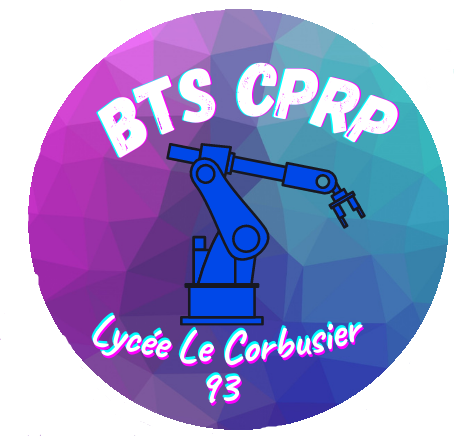
\includegraphics[width=0.2\linewidth]{btscprp.png}}
		\\ [2.0cm]
		\HRule{0.5pt} \\
		\LARGE TP1.4 Axes Machines \& architecture des MOCN \\ \textbf{DOCUMENT RÉPONSE}
		\HRule{2pt} \\ [0.5cm]}
\maketitle

\textbf{Deux personnes par groupe}\\ Toutes les questions seront traitées dans ce dossiers.


Nom :  \hspace{5cm} Prénom : \\


\vspace{1cm}

-----------------------------------  \hspace{1cm}   ---------------------------------

\vspace{1cm}

-----------------------------------  \hspace{1cm}   ---------------------------------




%\tableofcontents
%-------------------------------------------------------------------------------
% Section title formatting
\sectionfont{\scshape}




\newpage



%%%%%%%%%%%%%%%%%%%%%%%%%%%%%%%%%%%%%%%%%%%%%%%%%%%%%%%%%%%%%%%%
%%%%%%%%%%%%%%%% MACHINE 1 %%%%%%%%%%%%%%%%%%%%%%%%%%%%%%%%%%%%%
%%%%%%%%%%%%%%%%%%%%%%%%%%%%%%%%%%%%%%%%%%%%%%%%%%%%%%%%%%%%%%%%

\section{Généralités sur les MOCN}
\subsection{Machine 1}
\begin{exo}\label{exo1} A propos de la machine ci-dessous, rayer les mentions inutiles :
\begin{itemize}
    \item C'est une fraiseuse à commande numérique;
    \item C'est un tour à commande numérique;
    \item C'est une perceuse à colonne.
\end{itemize}
\end{exo}


\begin{exo}\label{exo1} Retrouvez les différentes axes, pièces et ensembles constituant la machine-outil à commande numérique et indiquez les numéros correspondants :\\ \end{exo}
\begin{minipage}{.55\linewidth}
\begin{itemize}
    \item Outil numéro x :
    \item Broche :
    \item Arrosage :
    \item Arrêt d’urgence :
    \item Magasin d’outils :
    \item Directeur de commande numérique :
    \item Porte de sécurité :
\end{itemize}

\end{minipage}
\begin{minipage}{.44\linewidth}
\begin{itemize}
    \item Porte de sécurité :
    \item Bac à copeaux :
    \item Étau :
    \item Axe X :
    \item Outil :
    \item Axe Z :
    \item Bâti :
\end{itemize}
\end{minipage}





%%%%%%%%%%%%%%%%%%%%%% FIN %%%%%%%%%%%%%%%%%%%%%%%%%%%%%%%%%%%%%%%%%%%%%%
%%%%%%%%%%%%%%%%%%%%%%%%%%%%%%%%%%%%%%%%%%%%%%%%%%%%%%%%%%%%%%%%%%%%%%%%%




%%%%%%%%%%%%%%%%%%%%%%%%%%%%%%%%%%%%%%%%%%%%%%%%%%%%%%%%%%%%%%%%
%%%%%%%%%%%%%%%% MACHINE 2 %%%%%%%%%%%%%%%%%%%%%%%%%%%%%%%%%%%%%
%%%%%%%%%%%%%%%%%%%%%%%%%%%%%%%%%%%%%%%%%%%%%%%%%%%%%%%%%%%%%%%%




\subsection{Machine 2}

\begin{exo}\label{exo1} A propos de la machine ci-dessous, rayer les mentions inutiles :
\begin{itemize}
    \item C'est une fraiseuse à commande numérique;
    \item C'est un tour à commande numérique;
    \item C'est une perceuse à colonne.
\end{itemize}
\end{exo}


\begin{exo}\label{exo1} Retrouvez les différentes axes, pièces et ensembles constituant la machine-outil à commande numérique et indiquez les numéros correspondants :\\ \end{exo}
\begin{minipage}{.55\linewidth}
\begin{itemize}
    \item Outil numéro x :
    \item Mors :
    \item Mandrin :
    \item Guide chariot vertical $\overrightarrow{x}$ :
    \item Contre-broche :
    \item Centre de commande / pupitre\\ de commande (IHM : Interface homme machine) :
    \item Porte de sécurité :
    \item Axe $\overrightarrow{X}$ :
    \item Bâti :
\end{itemize}


\end{minipage}
\begin{minipage}{.44\linewidth}
\begin{itemize}
    \item Magasin d’outils :
    \item Bac à copeaux :
    \item Marque du constructeur :
    \item Modèle du constructeur :
    \item Bouton d'arrêt d’urgence :
    \item Axe $\overrightarrow{Z}$ :
    \item Axe $\overrightarrow{C}$ :
    \item Axe $\overrightarrow{Y}$ :
\end{itemize}
\end{minipage}

\section{Fonctionnement des machines outils}
\begin{exo}\label{exo1} En vous aidant de la Figure indiquez d'où viennent les ordres de déplacement des machines outils.\end{exo}

\begin{tikzpicture}
\draw (0,0) -- (0,7) ;
\draw (0,7) -- (15,7) ;
\draw (15,7) -- (15,0) ;
\draw (15,0) -- (0,0) ;
\end{tikzpicture}

\newpage

\begin{exo}\label{exo1} Selon le diagramme Figure, de combien d'axe(s) dispose la machine outil  ?\end{exo}
\begin{tikzpicture}
\draw (0,0) -- (0,3) ;
\draw (0,3) -- (15,3) ;
\draw (15,3) -- (15,0) ;
\draw (15,0) -- (0,0) ;
\end{tikzpicture}



\begin{exo}\label{exo1} En vous aidant de la Figure : Que se passe-t-il si, lors d'une erreur de programmation d'usinage, un outil force sur la pièce ?\end{exo}
%% Si un outil force, le couple va augmenter jusqu'à détection du surcouple, la chaîne de sécurité sera alerté et l'automate,  par l'intermédiaire d'une signalisation et du contrôle du variateur, va pouvoir arrêter le processus en cours %%
\begin{tikzpicture}
\draw (0,0) -- (0,7) ;
\draw (0,7) -- (15,7) ;
\draw (15,7) -- (15,0) ;
\draw (15,0) -- (0,0) ;
\end{tikzpicture}

\section{Structures \& architectures des machines outils}


\begin{exo}\label{exo1} En rappelant le nom des machines outils sur lesquelles vous vous êtes rendus, indiquez si, d'après vous, elles font partie d'une structure type \textbf{ouverte} ou \textbf{fermée}.\end{exo}
\begin{tikzpicture}
\draw (0,0) -- (0,3) ;
\draw (0,3) -- (15,3) ;
\draw (15,3) -- (15,0) ;
\draw (15,0) -- (0,0) ;
\end{tikzpicture}

\newpage

\begin{exo}\label{exo1} Appelez votre enseignant, et inspectez si dans l'atelier de production, vous disposez de machine avec une structure en parallèle.\end{exo}
\begin{tikzpicture}
\draw (0,0) -- (0,3) ;
\draw (0,3) -- (15,3) ;
\draw (15,3) -- (15,0) ;
\draw (15,0) -- (0,0) ;
\end{tikzpicture}





\section{Système d'axe des machines outil}
\subsection{Définition}

\begin{exo}\label{exo1} Rappelez l'intérêt des normes dans l'industrie.\end{exo}
\begin{tikzpicture}
\draw (0,0) -- (0,7) ;
\draw (0,7) -- (15,7) ;
\draw (15,7) -- (15,0) ;
\draw (15,0) -- (0,0) ;
\end{tikzpicture}

\newpage

\begin{exo}\label{exo1} Recherchez la définition de la norme \textbf{AFNOR NF Z 68-020}, quel est son but ?\end{exo}
\begin{tikzpicture}
\draw (0,0) -- (0,7) ;
\draw (0,7) -- (15,7) ;
\draw (15,7) -- (15,0) ;
\draw (15,0) -- (0,0) ;
\end{tikzpicture}


\begin{exo}\label{exo1} En recherchant les informations de la norme \textbf{AFNOR NF Z 68-020}, définissez les notions suivantes :\end{exo}
%% http://philippe.berger2.free.fr/productique/ressources/origines/origines.htm %%
\begin{itemize}
    \item Un axe :
    \item Trièdre de référence : 
    \item Axe $\overrightarrow{Z}$ :\\
\end{itemize}


\begin{tikzpicture}
\draw (0,0) -- (0,7) ;
\draw (0,7) -- (15,7) ;
\draw (15,7) -- (15,0) ;
\draw (15,0) -- (0,0) ;
\end{tikzpicture}

\newpage

\begin{exo}\label{exo1} En recherchant les informations de la norme \textbf{AFNOR NF Z 68-021} (attention ce n'est plus la même), définissez les courses et origines suivantes (vous verrez que c'est assez subtile) :\end{exo}
\begin{itemize}
    \item $OM$ :
    \item $om$ :
    \item $Op$ :
    \item $Opp$ :
    \item PREF :
    \item DEC :
\end{itemize}


\begin{tikzpicture}
\draw (0,0) -- (0,7) ;
\draw (0,7) -- (15,7) ;
\draw (15,7) -- (15,0) ;
\draw (15,0) -- (0,0) ;
\end{tikzpicture}


\begin{exo}\label{exo66} Parmi les 6 éléments ci-dessus, entourez \textbf{en rouge} ceux qui, selon vous, sont des vecteurs (deux éléments attendus).  \end{exo}

\newpage

\begin{exo}\label{exo1} D'après vous, pour quelle raison principale nous avons eu besoin de définir autant de courses et origines différentes ? \end{exo}
\begin{tikzpicture}
\draw (0,0) -- (0,7) ;
\draw (0,7) -- (15,7) ;
\draw (15,7) -- (15,0) ;
\draw (15,0) -- (0,0) ;
\end{tikzpicture}
%% Sans ces différentes origines/courses, à chaque changement de pièces, outil, problème quelconque, nous devrions re-régler toute la machine outil. Grâce à elles, on peut facilement changer d'outil et ne changer qu'une seule valeur. Les différents jeu entre les pièces peuvent aussi constamment changer, c'est pourquoi nous avons besoin de beaucoup d'origines différentes. %%




\subsection{Comment dire à la MOCN où commencer votre programme ?}
\subsubsection{Le PREF}
%% http://robert.cireddu.free.fr/Progression/Formation%20en%20PRODUCTIQUE.html %%

\begin{exo}\label{exo1} Sur les deux figures ci-dessous (vue de coté et vue du dessus), inscrivez \textbf{en rouge} l'origine OP et tracez les distances $\overrightarrow{PREF_X}$, $\overrightarrow{PREF_Y}$ et $\overrightarrow{PREF_Z}$.\end{exo}
\begin{center}
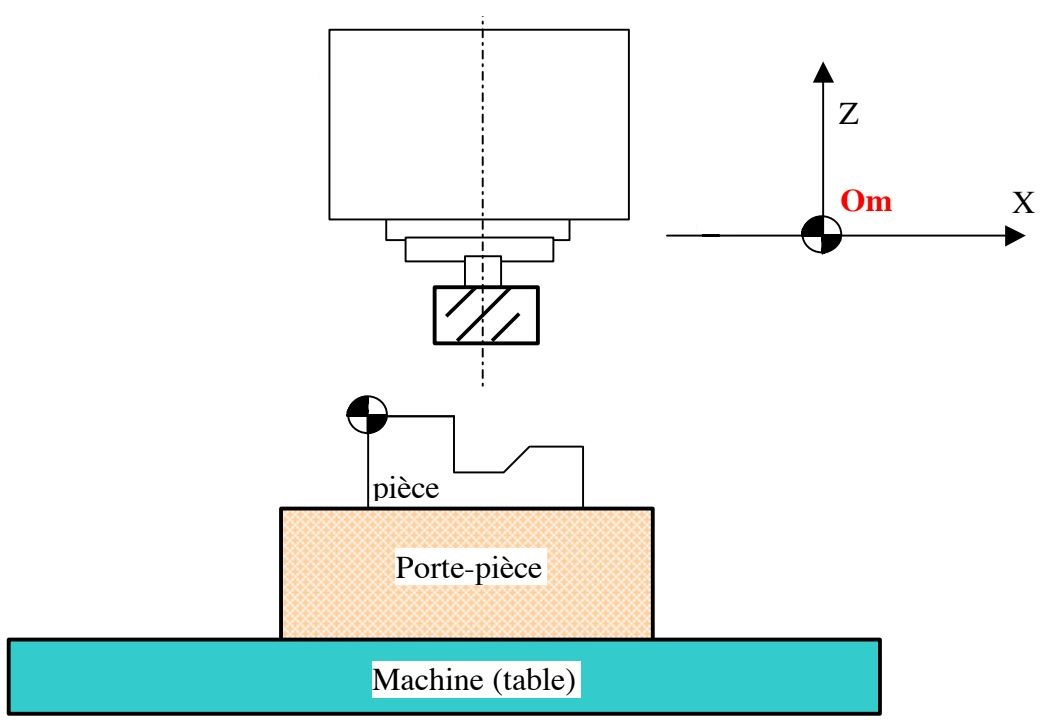
\includegraphics[width=0.8\linewidth]{OmOP1.JPG}
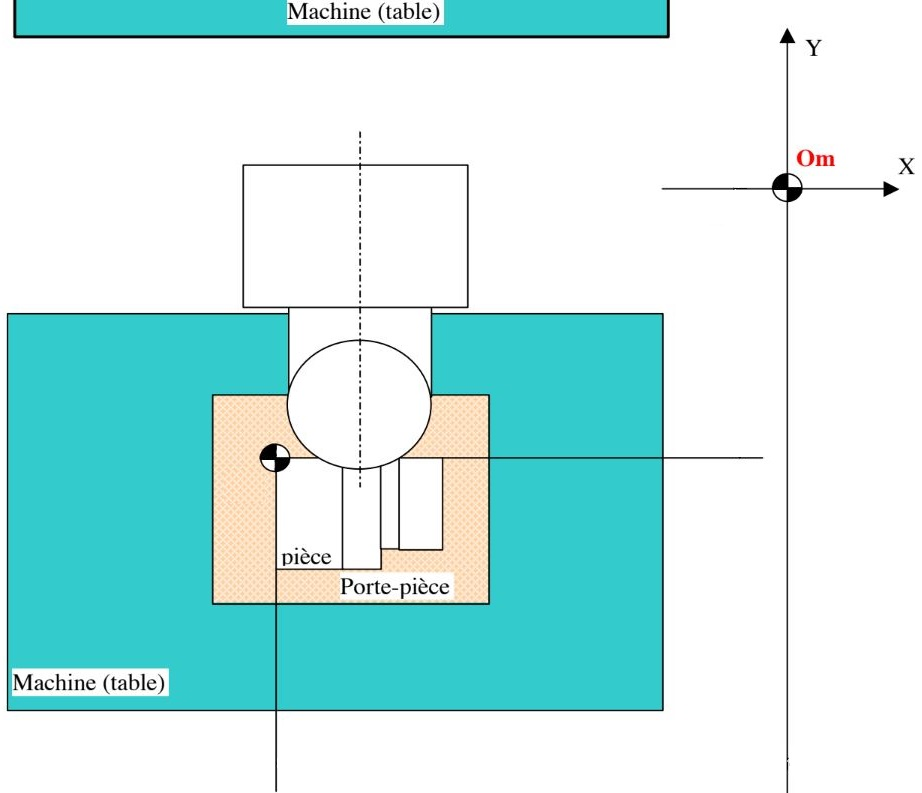
\includegraphics[width=0.8\linewidth]{OmOP2.JPG}
\end{center}

\subsubsection{Le DEC}

\begin{exo}\label{exo1} Sur les deux figures ci-dessous (vue de coté et vue du dessus), inscrivez \textbf{en rouge} l'origine OP et Opp et tracez les distances $\overrightarrow{PREF_X}$, $\overrightarrow{PREF_Y}$ et $\overrightarrow{PREF_Z}$ ainsi que les $\overrightarrow{DEC_X}$, $\overrightarrow{DEC_Y}$ et $\overrightarrow{DEC_Z}$.\end{exo}
\begin{center}
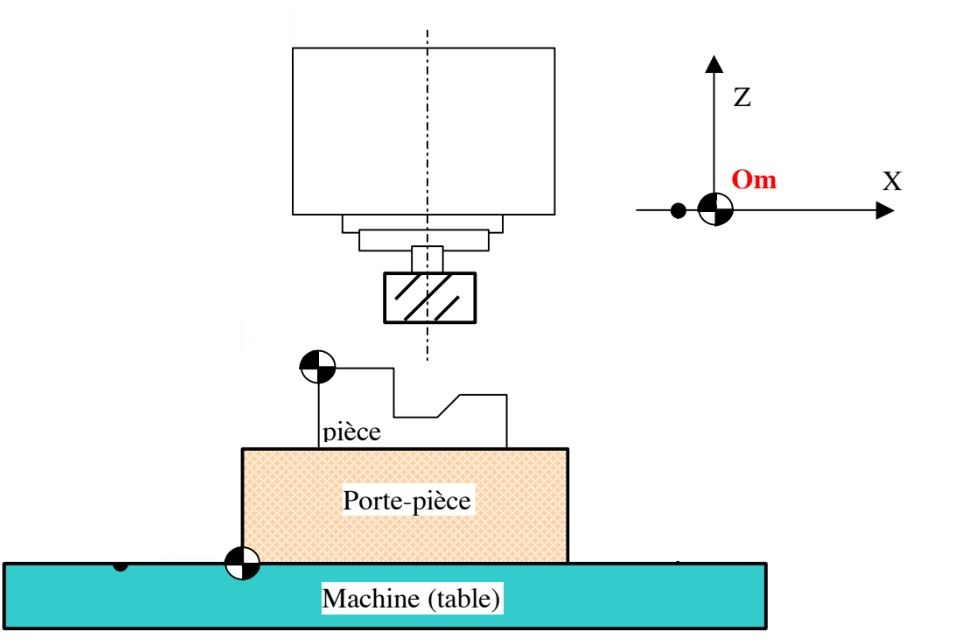
\includegraphics[width=0.8\linewidth]{DEC1.JPG}
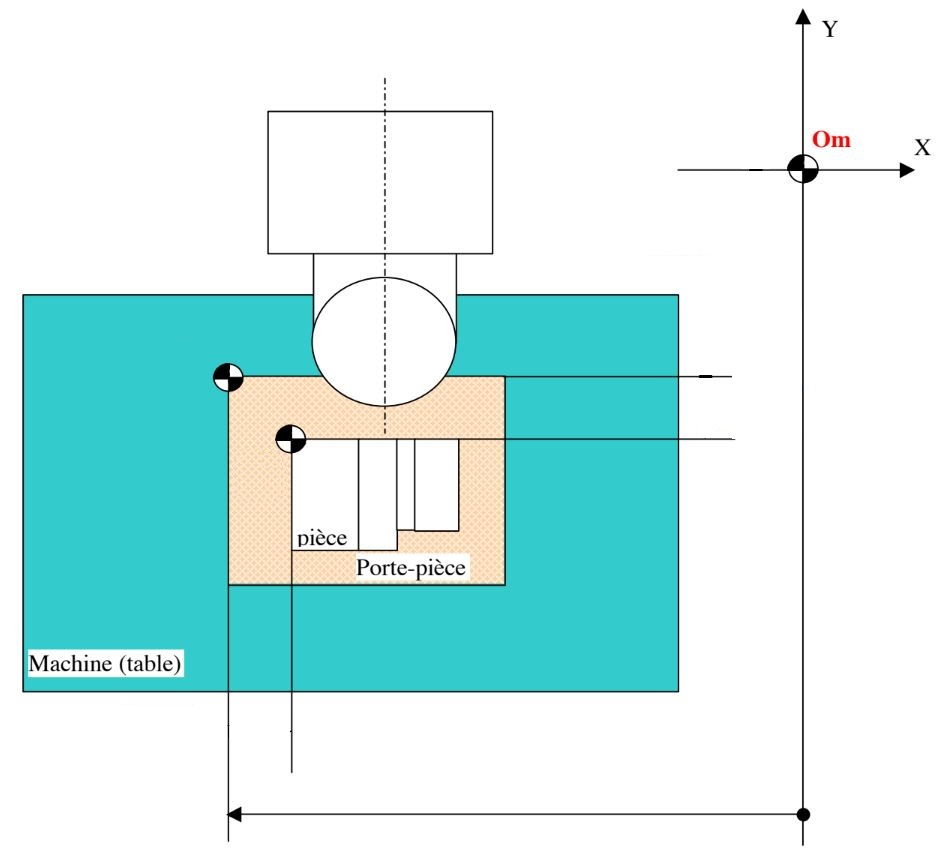
\includegraphics[width=0.85\linewidth]{DEC2.JPG}
\end{center}

\subsection*{En tournage}

\begin{exo}\label{exo1} Sur la figures ci-dessous, inscrivez \textbf{en rouge} les axes de la machine, l'origine \textbf{OP} et \textbf{Opp} et tracez les distances $\overrightarrow{PREF_X}$, $\overrightarrow{PREF_Y}$ et $\overrightarrow{PREF_Z}$ ainsi que les $\overrightarrow{DEC_X}$, $\overrightarrow{DEC_Y}$ et $\overrightarrow{DEC_Z}$.\end{exo}
\begin{center}
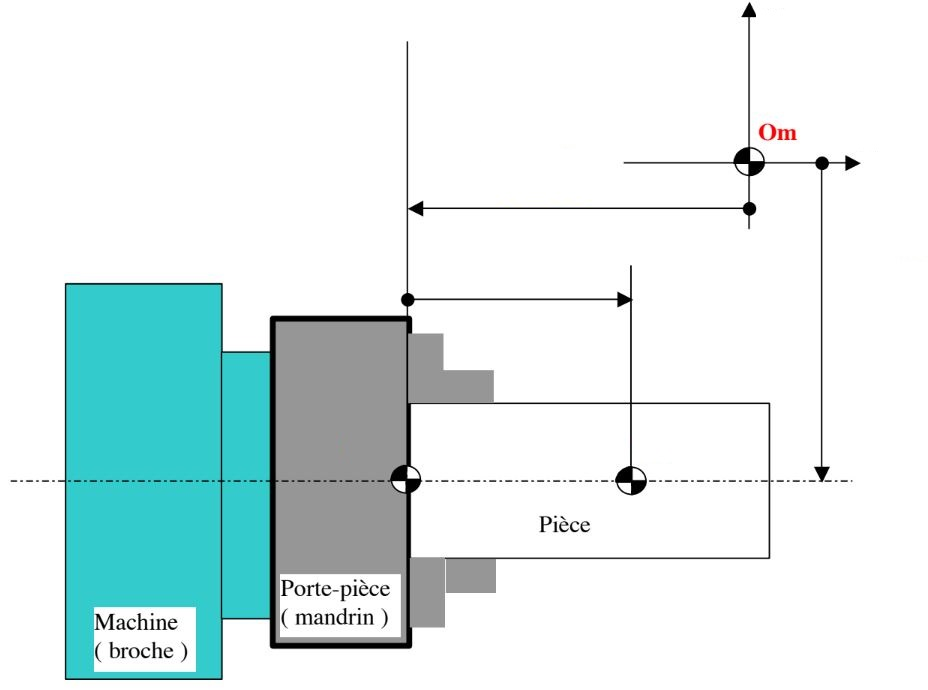
\includegraphics[width=0.9\linewidth]{PREFDEC1.JPG}
\end{center}


\subsection{Comment dire à la MOCN de quelles formes sont vos outils ?}

\subsubsection{Le cas du tournage}

\begin{exo}\label{exo1} Sur la figures ci-dessous, tracer \textbf{en rouge} les jauges des outils pour le cas d'un tour.\end{exo}
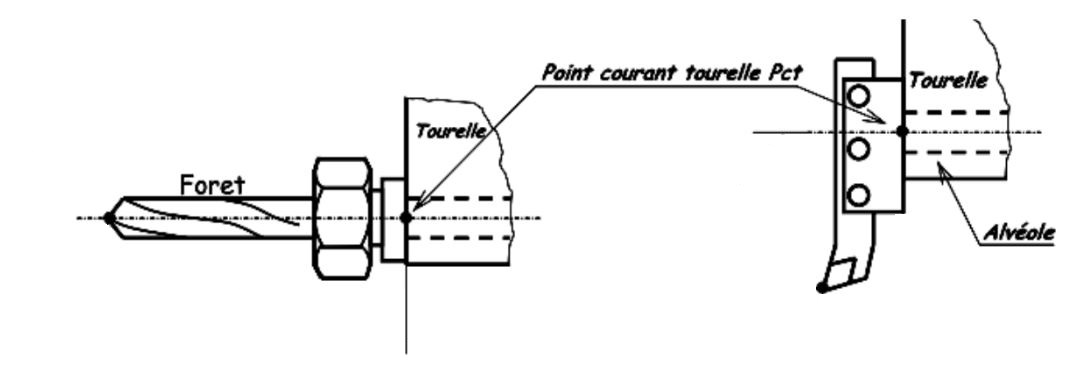
\includegraphics[width=1.05\linewidth]{jauge1.JPG}


\subsubsection{Le cas du fraisage}

\begin{exo}\label{exo1} Sur la figures ci-dessous, tracer \textbf{en rouge} les jauges des outils pour le cas d'un centre d'usinage.\end{exo}
\begin{center}
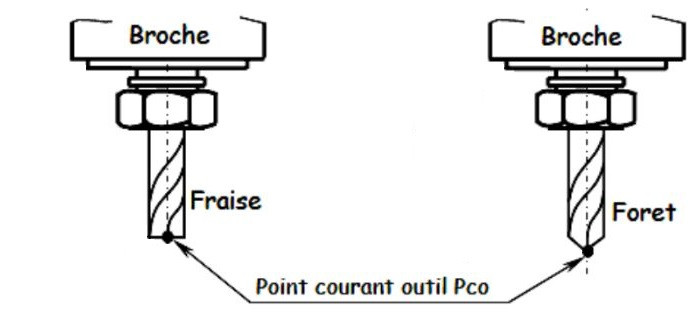
\includegraphics[width=0.8\linewidth]{jauge2.JPG}
\end{center}

\end{document}